\chapter{Overall Description}

\section{Product Perspective}
NonSoloLibri will be developed from scratch and will be a mobile application that runs on
both iOS and Android. 

Data will be stored online so that they can retrieved from every device and to provide a sort of back-up option.
Thus, users will be required to have a smartphone or tablet and a Google account to sign in.

In the application the users will be able to make use of their device hardware to capture pictures of books and libraries or to scan the book barcodes.

Verifying users will be mandatory in order to let them access to the market place, to security layer and discourage bad behaviours.

\section{Actors}

We individuated three main actors for the application:

\begin{description}
    \item[Visitor] A person who has yet to login to the application and can only see the login page.
    \item[User] A visitor who successfully logged in into the application and can access to all the main feature of the aplication.
    \item[Verified User] An user who successfully verified himself and can access to the market place.
\end{description} 

\newpage

\section{Use Cases Diagram}
The main actors have different functionalities, according to the previous definitions. \\
The visitior can only perform the login, the user can also make other things, like to manage the library or review a book.
Verified user can interact with the market functions.\\
All the functions are shown using the following use case diagram:
\begin{figure}[!ht]
    \centering
	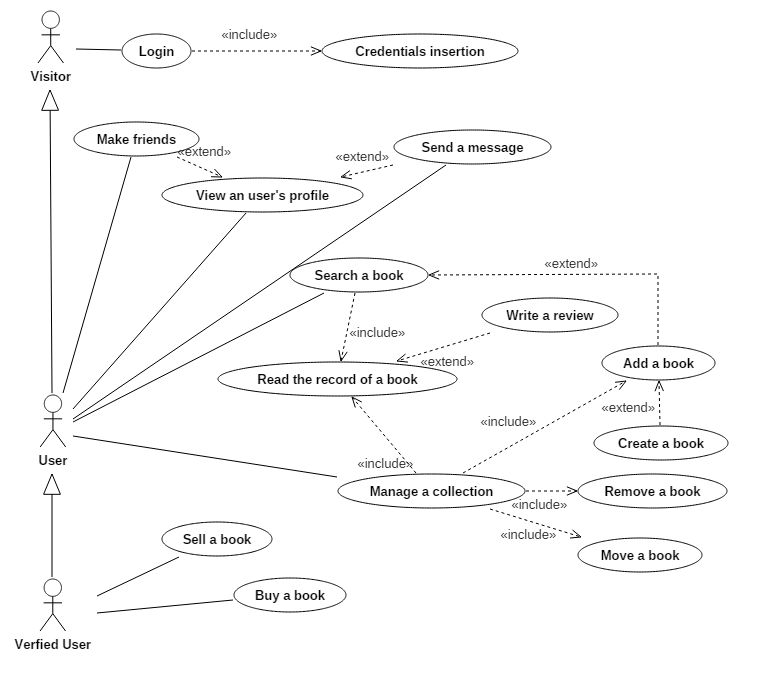
\includegraphics[scale=0.55]{images/use-case-diagram.png}
	\caption{Use case diagram}
	\label{fig:usecasediagram}
\end{figure}

\section{Product Requirements}
\begin{enumerate}
    \item Visitors should be able to login with their Google account.
    \item Users should be able to create libraries.
    \item Users should be able to edit libraries.
    \item Users should be able to customize libraries with photos or images.
    \item Users should be able to delete libraries.
    \item Users should be able to view libraries.
    \item Users should be able to add books to libraries.
    \item Users should be able to delete books from libraries.
    \item Users should be able to move books from a library to another.
    \item Users should be able to view books information.
    \item Users should be able to create books if they are not present in the database.
    \item Users should be able to suggest changes to books information.
    \item Users should be able to search for books in the database.
    \item Users should be able to send friendship requests.
    \item Users should be able to manage friendships.
    \item Users should be able to create a wish list.
    \item Users should be able to view their friends wish lists.
    \item Users should be able to verify themself.
    \item Verified users should be able to access to the market place.
    \item Verified users should be able to buy books in the market place.
    \item Verified users should be able to sell books in the market place.
\end{enumerate}

\section{Constraints}

\subsection{Hardware  and Software Constraints}
\begin{enumerate}
    \item To use the application, users are required to have a smartphone or a table. The device can have either Android or iOS 
        \begin{itemize}
            \item For Android the minimum supported versione is Android 5.0 Lollipop.
            \item For iOS the minimium supported version is iOS 10.
        \end{itemize}
    \item The application requires a device configured and able to connect to the Internet.
    \item The application requires a device with a photocamera.
\end{enumerate}

\subsection{Safety and Regulation Constraints}
\begin{enumerate}
    \item The system must guarantee data is protected and accessible only by its owner.
    \item The application must ask for user permissions to acquire, store and elaborate images from their devices.
    \item The system must complain with local laws.  
\end{enumerate}


\section{Domain assumptions}
\begin{enumerate}
    \item Administration tasks such as verification of the users and data checks on books inserted by users are made through an independent web-application whose design is not part of this document.
    \item Users should behave coherently and in respect of good manners.
    \item Users should type in correct information when adding a new book.
    \item A library is composed by: a name, a picture or an image and can be favourite or not.    
    \item A library can contain only one copy of a book.
    \item Multiple books with the same ISBN code can be located in different libraries.
    \item A book is characterized by: title, authors, publisher, release date, length, edition number, price and a ISBN code.
    \item The application will work as an intermediary between users for book trading, but transactions and shipment will happen outside of the application context.
\end{enumerate}

